\clearpage

\section{Introduction}

[TODO: Intention, hypotheses and results of the study]



Discussion centers on potential practical implications of the present results, as well as on prospects for future research.

\clearpage

\section{Background}

	\subsection{Motivation}
	
	[TODO]
	
	E-learning providers are looking to improve the learning experience of their users and make progress as effective as possible. 
During a typical learning session each learner is subject to a range of volatile emotional states that help or hinder their learning success. 
Several factors and stimuli, both internal and external, can influence emotions. 
When we take this knowledge about emotions into account a new way to manage a learning session opens. We can incorporate this knowledge into learning sessions and provide a more appropriate task and interface for the learner.

The goal of the paper is to examine a relationship between the emotional aspect of a user interface in an e-learning system and its effect on the performance of the learner.


\begin{center}
	
\includegraphics[width=200px]{graphics/relation1.png}
\end{center}
 
There is strong evidence of the surrounding environment having an influence on emotion \cite{Johnson2000, Arockiam2013, Bertamini2013}. This includes, for example, an e-learning system on the screen in front of the learner. In a similar fashion several studies have shown a correlation between emotion and cognition (Section \ref{sec:emotion-cognition}).

\begin{center}

\includegraphics[width=300px]{graphics/relation2.png}
\end{center}

There is a logical argument of the existence of a transitive relation between these parameters, which could confirm the dependency of the edge variables. 
I.e. exposure to several interfaces each with a different emotional charge during an on-line lesson should lead to a difference in performance when working on the same task.
Insufficient research confirming this connection and explaining the effects has been published yet. 

In this paper I would like to explore to which extent the final parameter "learning success" can be influenced with the limited surface of contact that can be addressed through a learning interface on the screen.
	
		
	\subsection{Research basis} \label{sec:research}
	
	Information architecture and display types play an important role in learning comprehension, attention and learning success. \cite{McCrudden2017} describe the effects of different types of visual display on cognitive processing. They highlight the important aspects of visual guidelines, the basics of human understanding and  memory, as well a way to quantify those under processing efficiency. One of their conclusions is that "displays should be designed to support the selection of important information" \cite[p.633]{McCrudden2017}
	
	There is, however, a case to be made with respect to the same visual display that can be put forth in front of participants under differentiating emotional conditions. There is strong evidence that emotions play a role in information processing and, as a consequence, can have an effect on the resulting performance. Section \ref{sec:emotion-cognition} discusses closer existing research of a connection between emotion and cognition
	
	A recent study \cite{Haaranen2015} suggests that wrong choice of emotional design patterns can yield contra-productive results. It reports lover concentrations levels in the experiment group compared to control group using abstract graphics when learning object-oriented programming (OOP). Due to their choice of presentation and the topic or learning, the material has not been perceived as serious and a such became distracting.
		
		\subsubsection{Emotion theory}
		
		[TODO]: summarize Valence-Arousal model and explain 4 groups
		
		\subsubsection{Emotion and cognition} \label{sec:emotion-cognition}
		
		A 2004 cognitive neuroscience study \cite{Dolcos2004} scanned participants brain activity, while rating emotional pictures. The study suggests several relevant conclusions. First, that different parts of the brain show stronger activity when exposed to positive compared to negative stimuli. Second, that high arousal stimuli lead to greater successful encoding activity, or in other words - rate of recall, than neutral stimuli. 
		
		In other words, brain response is different for arousing stimuli of positive valence compared to negative valence. Furthermore memory is mediated, in part by both - valence and arousal levels. It provides basis to the assumption that variation on both dimensions is necessary to adequately reflect effects within e-learning context. Study design in \ref{sec:study-design} depends heavily on this assumption.
		
		\subsubsection{Emotion and visual interface}
		
		\cite{Desmet2007} demonstrates in their research that physical objects can cause significant emotional response and that modifying design attributes can successfully contribute to creating of desired response.
		Both physical objects and digital visuals are, in essence, interfaces. Both can cause an emotional response \citationneeded Digital interfaces are extremely flexible to experimentation and modification at low cost.
	
	\subsection{Hypotheses}
	
		\paragraph{Hypothesis 1.} Two different interfaces can result in a significant difference in emotional response
		\paragraph{Hypothesis 2.} Resulting performance (as measured by selected study design parameters) during the experiment is higher for saturated interface, compared to desaturated interface.

\section{Approach and Methods}

To facilitate the study I make assumptions about the medium in which e-learning is usually conducted. Based on research basis (\ref{sec:research}) I define study design parameters and a set of target variables that are evaluated.

	\subsection{Medium}
	
	The study is to be conducted online under a "real-life" scenario. This means, that the experiment is to be run in a browser-capable web-application runnable on modern personal computers. Like most e-learning software the  application used in the study is browser-based and usually used in users homes or public places.
	
	\subsection{Study design} \label{sec:study-design}
	
	Goal of the current study is to determine emotional response to provided emotional design implementation (Interface 1) compared to the control group that is provided with a stricter desaturated design (Interface 0). Differences include use of color, shapes, language, font style, interaction responsiveness, animation. The similarities or - constant variables - across both interfaces include any accessibility features and general usability heuristics, such as contrast ratio level, size and placement of elements on a screen.
	
	The experiment can be outlined and split into following steps:
	
	\begin{enumerate}
		
		\item[0.] \textbf{Clustering:} Each participant is assigned an interface version (1 of 2) and the preconditioning group (1 of 4) at random before first load of the application.
		
		\item \textbf{Preconditioning:} Each participant is shown a set of emotional images and preconditioned to be in one of 4 states:
			\textbf{1}: Positive valence / high arousal;
			\textbf{2}: Negative valence / high arousal;
			\textbf{3}: Positive valence / low arousal;
			\textbf{4}: Negative valence / low arousal;
			
		Choice of stimuli and their presentation is described further in chapter \ref{preconditioning}
			
		\item \textbf{Emotional report:} A short emotional self-reporting questionnaire (SAM \ref{sec:selfeval}) is used to validate, whether preconditioning has had sufficient and expected effect on the participant.
		
		\item \textbf{Experiment 1:} Slightly modified classic memory game. The participant is presented with a grid of tiles, each tile containing an image. During 5 seconds at the beginning of the experiment all tiles are open to allow to memorize the images. After which all images are hidden. Only 2 tiles can be opened at any one time. Once 2 of the same tiles are open they are marked as solved. The goal is to solve all tiles.
		
		\item \textbf{Experiment 2:} Remote Associates Test (RAT). A generalized creativity test developed by Mednick \cite{Mednick1962} in 1962. Each participant is presented with a number of word sets. Each set consists of 3 words that are shown to the participant and one target word that is hidden from the them. The target word is semantically connected to all 3 visible words
		
		\item \textbf{Emotional validation:} A second emotional self-reporting questionnaire (SAM \ref{sec:selfeval}) is used to establish, whether and which effect tasks and interface have had on the participant's emotion.
		
		\item \textbf{Demographic data:} Final step adds additional personal context data for each participant through a questionnaire to complement data analysis (discussed in \ref{sec:demographics}).
		
	\end{enumerate}
	
	\subsection{Preconditioning sequences} \label{preconditioning}
	
	\paragraph{Finding a preconditioning sequence}
To facilitate emotional conditioning I selected a specialized sequence containing images with a corresponding emotional charge.
Each sequence contains 21 to 39 \todo{more precise} images with each displayed for about 5 seconds.

Each subject is assigned one of four preconditioning sequences. Each sequence is aimed to condition the subject into one of the 4 quadrants, described though a valence-arousal emotional model. To simplify we will label (\ref{fig:valence_arousal_model}) them as:
\begin{enumerate}
	\item Angry (Quadrant 1)
	\item Happy (Quadrant 2)
	\item Sad (Quadrant 3)
	\item Relaxed (Quadrant 4)
\end{enumerate}


\begin{figure}
\begin{center}
	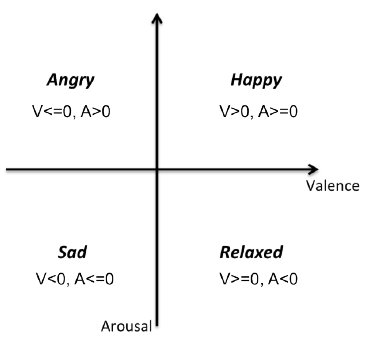
\includegraphics[width=150px]{graphics/Valence-Arousal-model-showing-the-quadrants-of-the-four-emotion-tags-used-in-this_W640.jpg}
	\caption{Valence Arousal Model \cite{Song2013} \label{fig:valence_arousal_model}}
	
\end{center}
\end{figure}

There are several emotional image data-sets available for academic purposes such as GAPED \cite{Dan-Glauser2011}, OASIS \cite{Kurdi2017}, IAPS \cite{Lang1997} and NAPS \cite{Marchewka2014}. While NAPS is offering the highest realism and quality of images, the range images seems to cover "sad" and "happy" to a less pronounced degree. In general, strong negative valence values are accompanied with high arousal values across all analyzed data-sets. Causing sadness is a challenging task. In current preconditioning sequences I am using the \textbf{OASIS} database. It has relatively wide spread of emotions compared to other sets.

Keeping in mind the need for a clear separation between groups in terms of their emotional state into account, I limited emotional images to moderately strong stimuli values, thus avoiding extreme reactions and unrealistic emotional states. It can be assumed that in most cases, people who attend e-learning lessons will have moderate levels of emotional charge. It is important to note that quadrant 1 - angry and quadrant 2 - happy has a more pronounced representation in emotional databases due to an easier and more prevalent stimuli availability. As such quadrant 1 and quadrant 2 have stronger stimuli compared to quadrant 3 and 4. It is expected that there will be a significant difference between emotion ratings of participants across these groups.

It is understood that the e-learning interface under real conditions will only cause mild-to-moderate changes to a mood.


\begin{figure}
	\centering
	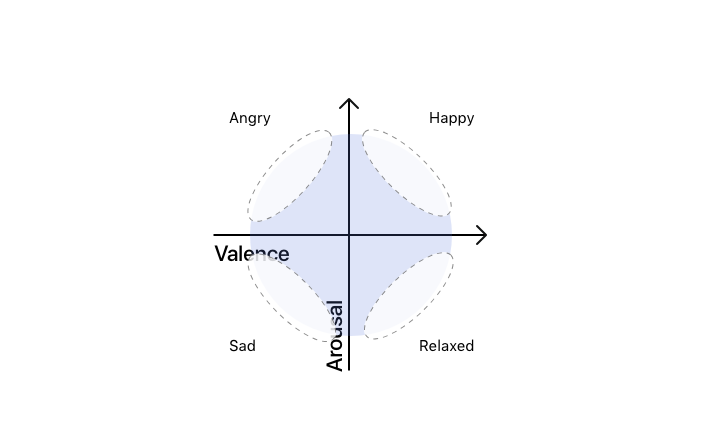
\includegraphics[width=0.7\linewidth]{graphics/Valence-Arousal-Model-1.png}
	\caption{Focus levels of emotional states on valence arousal model}
	\label{fig:valence-arousal-model-2}
\end{figure}

Illustration \ref{fig:valence-arousal-model-2} highlights with dashed outline areas the target arousal and valence values

	
	\subsection{Emotional Design Features}
	
	[TODO:] write about emotional design, rewrite citation blocks below
	
	\clearpage

\paragraph{Developing a high performing interface}

There is a multitude of studies that analyze user interface design and user emotion. In following I will summarize them in respect to UI features tailored towards high performance

\paragraph{Literature review}

A paper by L. Arockiam et al \cite{Arockiam2013} describes that, based on previous research and their own findings optimal ui can be achieved based on a person's personality traits. We will limit ourselves to a universal set of changes that should evoke high arousal, positive valence and therefore have an effect on learning outcome, rather than look for their preference. Nevertheless it is worth mentioning...

Color - PHYSIOLOGICAL

Wilson (1966) reported higher GSR measurements for red as opposed to green, and Nourse and Welsh (1971) reported higher GSR readings for violet than green. Using 24 male college students as subjects and saturated samples of red, yellow, green, and blue as stimulus materials, Jacobs and Hustmyer (1974) found that red was significantly more arousing than either yellow or blue, and green more than blue. Using 40 undergraduate students as subjects, Jacobs and Suess (1975) found that red and yellow resulted in higher anxiety state scores than blue or green when measured by the StateTrait Anxiety Inventory. Bloomer (1976) also reported that red increases heart rate. There appears to be some evidence that spectral extremes, especially red, cause greater arousal than mid-spectral colors. This may relate to the fact that wavelengths at the extremes of the spectrum, such as red and violet, focus at different points in the eye than wavelengths at the middle of the spectrum. \cite{Pert1996}

Color - PSYCHOLOGICAL

The selected order of preference was: (1) blue, (2) red, (3) green, (4) violet, (5) orange, (6) yellow. This selection agreed with the average rankings of color preference among 21,060 subjects reported in earlier investigations. The order was the same for all races and for men and women with one exception. Men chose orange over yellow whereas women chose yellow over orange. \cite{Pert1996}

no significant differ- ences between men and women or between subjects of different races.\cite{Pert1996}

girls of all ages preferred higher value, brighter, colors as compared to boys (Child, et al., 1968) \cite{Pert1996} (study among school age children from 1 to 12 grade)

Results on the evaluation scale supported the general preference for cool colors(bl~e and green) as compared with warm colors(red and yellow) and agree with previous findings by Adams and Osgood (1973) that red is a potent color while gray and black have low potency. \cite{Pert1996}

In a color-effectiveness study conducted at Fort Monmouth, typical army training procedures were used with 11 different television lessons (Kanner and Rosenstein, 1960). No significant
differences were found in learning between
monochrome and colored versions \cite{Pert1996}

Schaie (1966) pointed out that color prefer-
ences vary from individual to individual and relate to personality. \cite{Pert1996}

(so far black and white and color has not yielded any significant difference in learning) but "colored mate- rials are preferred by learners." \cite{Pert1996}

1972: those who viewed colored transparencies had had a more positive attitude toward transparencies than \cite{Pert1996}

In a research study on color coding, Lamberski and Dwyer (1983) concluded that color is an attention-getting device that can provide measurable effects on learning that cannot be accounted for by words and labels. \cite{Pert1996}

Search Tasks: 
gain in efficiency, indicated by decreased search time, with codes of up to five colors \cite{Pert1996}

Color was found to be useful in grouping information

color versions resulted in higher recognition- memory scores (immediate recognition memory test)\cite{Pert1996}

as the variable of visual complexity increases, so does the degree of recall. (Berry (1991a)) \cite{Pert1996}

The key factor relating to color and cogni-
tive learning seems to be that it is of value when it emphasizes relevant cues, is used as a coding device, or when it is a part of the con- tent to be learned (Dwyer and Lamberski, 1982- 83; Levie, 1973; Pruisner, 1993; Wedell \& Alden, 1973). \cite{Pert1996}

Non-objective Measures

(Scanlon, 1970). Scanlon suggests that the color versions (Grey Cup football game) create emotional effects that detract from attention to details.







Colors at the ends of the spectrum, red and
violet, seem to result in greater arousal, and
colors in the middle of the spectrum, yellow,
green, cyan, seem to be best for discriminating
detail. \cite{Pert1996}
	
	\subsection{Experiments}

		\subsubsection{Experiment 1: Short term Memory} \label{sec:memory}
		
		Memory Experiment 
		
		[TODO:] Describe basis of the experiment
		
		[TODO:] describe activity logging for EXP1 here?
		
		[TODO:] measuring performance of this experiment
		
		\paragraph{Performance parameters:} \label{sec:memory-parameters}
		
		\subsubsection{Experiment 2: Creative thought} \label{sec:creativity}
		
		A generalized creativity test developed by Mednick \cite{Mednick1962} in 1962. It does not require prior knowledge of any particular subject. Some of 144 compound remote associate sets are taken from \cite{Bowden}. These are a subset of RAT problems and have been alternatively described as "compound word problems". Of the triad of words that are presented each can form a compound word or a two-word phrase with the solution word.
		
		[TODO:] describe activity logging for EXP2 here?
		
		[TODO:] measuring performance of this experiment


	\subsection{Means of emotional self-evaluation} \label{sec:selfeval}
	
	

% \todo[inline, size=\tiny]{'Valence and Arousal evaluation techniques'}


	
	[TODO:] Describe Valence and Arousal evaluation techniques
	
	SAM , AS, Affect Grid \cite{Russell1989}
	
	Due to effort constraints of the participants it is important to achieve a simple, yet accurate reading of their emotions. In the context of this study self-evaluation is a means to validate results, of Hypothesis 1. I chose to rely on the proven SAM (Self-Assessment Manikin) method \cite{Bradley1994} to quickly allow users to assess their emotions on a dual 9 element scale.
	
	\subsection{Demographic data} \label{sec:demographics}
	
	As final step of the study each participant fills out a demographics questionnaire to add context data and help with analysis. There are 4 questions:
	
	\begin{itemize}
		\item Gender [Male / Female]
		\item Age [18-24 / 25-29 / 30-34 / 35 - 44 / older]
		\item Is English your native language? [yes / no]
		\item Occupation: [High school student / Undergraduate Student / Graduate Student / Doctorate / Professional or Working
	\end{itemize}

	The age groups are taken in accordance with suggestions provided by the Standard International Age Classifications \cite{UN1982} with slight modifications to exclude ages below 18. Further the study would focus on ages up to 44. Ages above 44 could potentially skew results due factors not considered by present study. Primary focus audience lies between ages of 18 and 34.
	
	Last field allows the user to enter their email address for participation in the raffle and complies with the motivational promise at the start of the study.

	\subsection{E-learning activity logging}
	
	To assess performance of subjects continuous measurements are taken during the test. General approach is an event based system where each action from the user or the system is emitted to the database. I differentiate between a "click" action that is initiated by the user and an "event" action that is generated by the EVAluation system
	%To assess performance of subjects several measurements are taken during the test, these differentiate between the 2 experiments.
	
	Describe general approach to recording actions and recording approach for this study.
		
		\paragraph{Current implementation} -
		
		[TODO:] describe how I implemented tracking, storage and analysis for current study
		
		\paragraph{xAPI adaptation} - 
		
		[TODO:] explore adaptability and possible constraints

\section{Study implementation}

\paragraph{Participant sourcing} 
This study includes participants attained through multiple sources:
\begin{itemize}
	\item{Local university:} On-site supervised experiments were conducted on a limited scale to facilitate a clean sample of participants and uncover problems during the study
	
	\item{Local workplace:} On-site semi-supervised experiments are conducted on a limited scale in Berlin area in Germany to facilitate a more diverse sample while keeping controlled environment conditions, similar to university experiments.
	
	\item{Social media:} Remote participants are invited to participate in unsupervised experiments on their own. Channels such as social media, interest groups and university mailing lists are used.
	
	\item{Mechanical turk:} MTurk is one of popuar web services to source participants. Previous research has shown that it can be considered a reliable platform for conducting objective studies. MTurk participants receive monetary compensation for participation \cite{Buhrmester2011a}. Mturk participants are excluded from motivation with a chance on winning a voucher prize (they do not see the field and information box about it), instead regular participant reward through MTurk is used.
	
\end{itemize}

Local and social media experiments provided additional motivation of participation with the promise of a chance to win a 20 Euro Amazon-voucher.

\paragraph{Technological implementation} is guided by the requirement to run the study in a browser on a personal computer. React.js is selected as a library of choice due to it's favorable characteristics to creating an environment that supports 2 themes and global settings in a scalable way. Reacts unidirectional data flow
allows clear behavior path between application data and visual representation. For example changing the theme in a global context propagates new style and visual rules applied throughout the application without losing current state.

\section{Results and Evaluation}

[TODO:] Here describe how evaluation was done, how many people participated, demographics data.

[TODO:] Show general statistical data

	\subsection{Hypothesis 1}: 
	
	[Note:] H1 should be checked in the context of the whole app
	
	\subsection{Hypothesis 2}: 
	
	[Note:] H2 should be checked for each task separately

\section{Further research and implications of the study}

\subsection{Ethical, legal and social implications}

[TODO]

\section{Notes}




